\documentclass[a4paper,12pt]{article}
\usepackage[utf8]{inputenc}
\usepackage{amssymb}
%\usepackage{polski}
\usepackage[polish]{babel}
\usepackage[T1]{fontenc}
\usepackage[utf8]{inputenc}
\usepackage{mathtools}
\usepackage{amsmath}
\usepackage{mathtools}
\usepackage{amsthm}
\usepackage{graphicx}
%\usepackage{marginnote}
\usepackage{l3keys2e}
\usepackage{array}
\usepackage{pgfcore}
\usepackage{tikz}
\usetikzlibrary{positioning}
\usetikzlibrary{arrows.meta}
\usetikzlibrary{arrows}
\usetikzlibrary{shapes.geometric}
\newcommand{\midarrow}{\tikz \draw[-triangle 90] (0,0) -- +(.1,0);}
%\usepackage{nicematrix}
\usepackage{tabularx}
%\usepackage{multirow}
%\usepackage{enumitem}


\title{\bf 12. Obliczanie całek $ \iint\limits_D f(x,y)\,dx\,dy $, gdzie $ D = [a,b] \times [c,d] $ złożoną kwadratururą Simpsona ze względu na zmienną $ x $ oraz złożoną kwadraturą prostokątów (z punktem środkowym) ze względu na zmienną $ y $ }
\author{Sebastian Szarafin \\ 313460}

\begin{document}
\maketitle

\section{Wstęp}
Kwadratury Newtona-Cotesa są prostymi za równo w zrozumieniu jak i w implementacji metodami przybliżającymi całkę funkcji ciągłej na zadanym przedziale. Niemniej jednak, przy odpowiednim doborze parametrów mogą być one całkiem dokładne. \\
W raporcie została zbadana metoda obliczania całek podwójnych funkcji $ f(x,y) $ opierająca się na połączeniu 2 złożonych kwadratur Newtona-Cotesa: kwadratury Simpsona względem zmiennej $ x $ oraz kwadratury prostokątów (z węzłem środkowym) względem zmiennej $ y $, na prostokącie $ D = [a,b] \times [c,d] $. \\
Jak się okazało, nawet przy względnie skomplikowanych funkcjach, wyniki odbiegały bardzo nieznacznie od wyników teoretycznych.

\section{Opis użytych metod}
Kwadratury na których bazuje omawiana metoda przybliżają całkę funkcji $ f(x) $ na przedziale $ [a,b] $ podzielonym na podprzedziały \\
 $ [x_{k-1},x_{k}] $ $ (k=1,...,N) $, o długosci $ H=\frac{b-a}{N} $. 
 
 \subsection{Kwadratura Simpsona}
%\vskip6ex \hfill \break lub \begin{flushleft}
Prosty wzór Simpsona, zwany również wzorem parabol jest oparty na węzłach: $a$ , $b$ i $ \frac{a+b}{2} $. Polega na przybliżeniu funkcji $ f $ wielomianem stopnia 2 i wyraża się wzorem:
\[
S(f)=\frac{b-a}{6} \left(f(a)+4f(\frac{a+b}{2})+f(b) \right). 
\]
Złożony wzór Simpsona ma postać:
\[
S(f)=\frac{H}{6} \left(f(a)+f(b)+2\sum_{k=1}^{N-1} f(a+kH) \hskip0.5ex + 4\sum_{k=0}^{N-1} f(a+kH+\frac{H}{2}) \hskip0.5ex \right),
\]
a jego błąd jest równy:
\[
E(f)=-\frac{1}{180 \cdot 2^4}H^4(b-a)f^{(4)}(\mu_2).
\]
Kwadratura Simpsona jest dokładna dla wszystkich wielomianów stopnia nie przekraczającego 3.

 \subsection{Kwadratura prostokątów}
 Prosty wzór prostokątów oparty jest na 1 węźle $ x_0 \in [a,b] $. Polega na przybliżeniu funkcji $ f $ wielomianem stopnia 0 i wyraża się wzorem:
 \[
 S(f)=(b-a)f(x_0).
 \]
Złożony wzór prostokątów (oparty na węźle środkowym) ma postać:
\[
S(f)=\sum_{k=1}^{N} (x_k-x_{k-1}) \hskip0.5ex f(\frac{x_k+x_{k-1}}{2}),
\]
a jego błąd jest równy:
\[
E(f)=\frac{1}{24}H^2(b-a)f''(\mu_3).
\]
Kwadratura prostokątów jest dokładna dla wszystkich wielomianów stopnia nie przekraczającego 1.

\section{Eksperymenty}
Metoda została przetestowana na kilku bardziej i mniej skomplikowanych funkcjach o różnorodnych przebiegach na zadanym przedziale. 

\vskip4ex
\subsection{Przykład 1}
Przykład 1 przedstawia przybliżenie całki $ \int\limits_{-10}^{10} \int\limits_{-15}^{15} x+y\,dx\,dy $. \\
Wykres przybliżanej funkcji przedstawia Rysunek 1.
\vskip2ex
\begin{figure}[!h]
\centering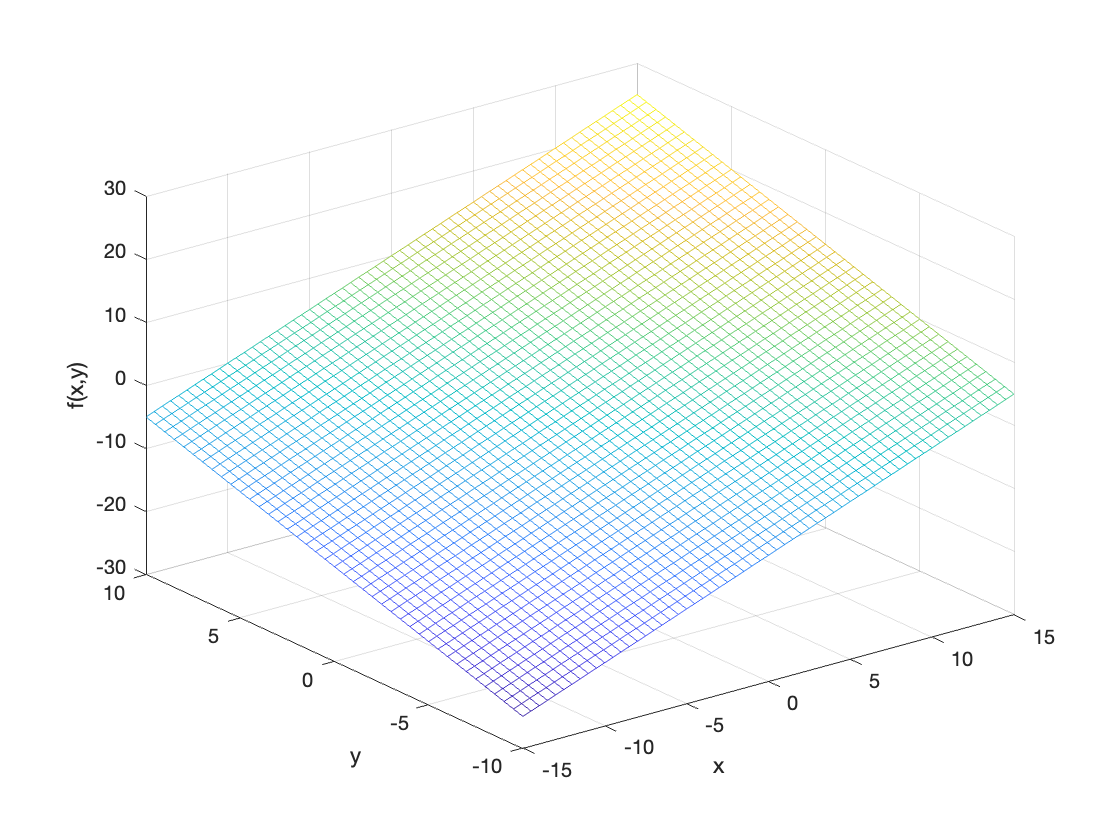
\includegraphics[width=10cm]{przyklad1.png}
\vskip-1.5ex
\caption{Przedstawia wykres funkcji $ f(x,y)=x+y $.}
\end{figure}
%\nopagebreak

 \begin{flushleft} Funkcja jest nieparzysta na zadanym przedziale, wobec tego jej całka jest równa 0. \\
Wyniki przybliżania przedstawiono w Tablicy 1. \end{flushleft}

\vskip-3ex
\begin{table}[h!]
\caption{Wyniki - Przykład 1} \vskip1ex
\renewcommand{\arraystretch}{1.1}
\centering\begin{tabular}{|c|c|c|c|c|}
\hline 	$N$ 		&	$ M $	&	 wynik uzyskany 	& 	wynik teoretyczny	&	błąd  			\\
\hline 	1 		& 	1 		& 	0 				&	0				&	0				\\
\hline 	10 		& 	10 		& 	0 				& 	0				&	0				\\
\hline 	100 		&	100 		& 	$1.8189e\!-\!14$ 	& 	0				&	$1.8189e\!-\!14$	\\
\hline 	1000 	& 	1000 	& 	0 				& 	0				&	0				\\
\hline 	10000 	& 	10000 	& 	$-1.1641e\!-\!16$ 	& 	0				&	$-1.1641e\!-\!16$	\\
\hline
\end{tabular}
\end{table}

\hfill \break 
Widać, że funkcja została bardzo dokładnie przybliżona, całka w 3 przypadkach jest równa dokładnie 0, a w 2 przypadkach jest bardzo bliska 0. Zwiększenie ilości podprzedziałów nie do końca przełożyło się na poprawę dokładności obliczeń, aczkolwiek uzyskane błędy są bardzo niewielkie i właściwie pomijalne. 

\subsection{Przykład 2}
Przykład 2 przedstawia przybliżenie całki $ \int\limits_{-3}^{3} \int\limits_{-3}^{3} x^2+y^2\,dx\,dy $. \\
Wykres przybliżanej funkcji przedstawia Rysunek 2.
\vskip2ex
\begin{figure}[!h]
\centering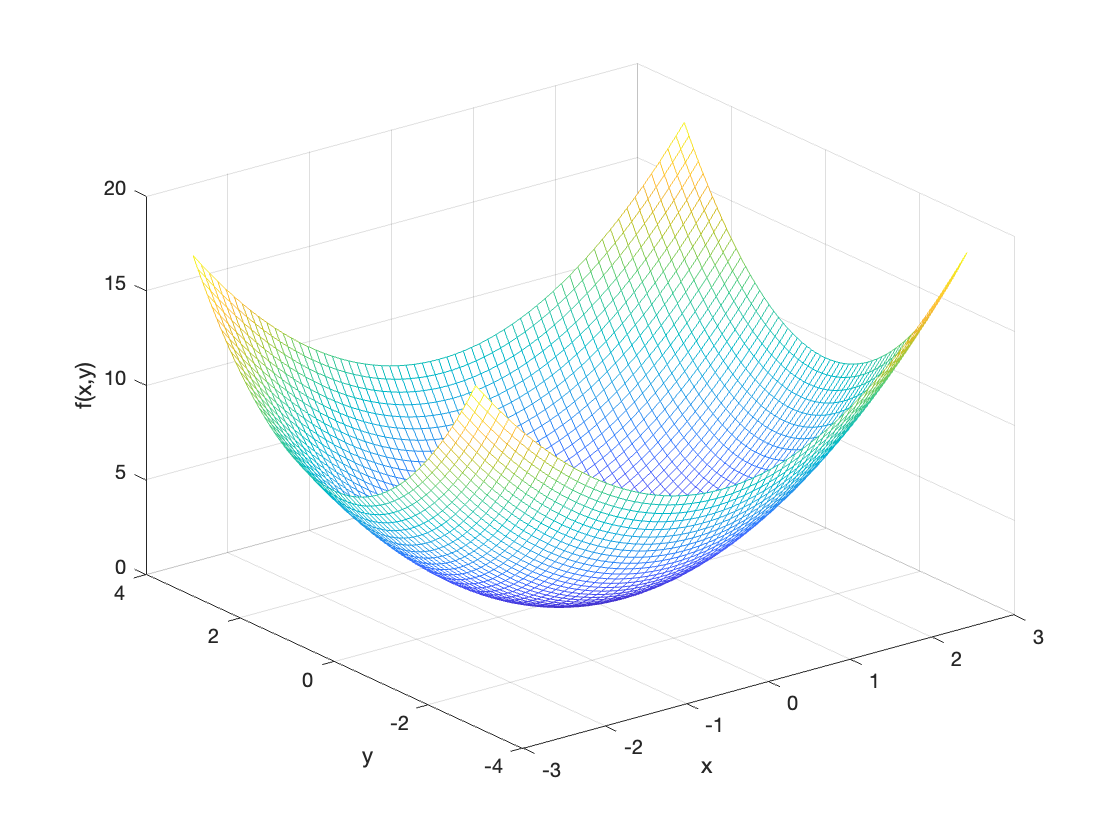
\includegraphics[width=10cm]{przyklad2.png}
\vskip-1.5ex
\caption{Przedstawia wykres funkcji $ f(x,y)=x^2+y^2 $.}
\end{figure}
%\nopagebreak
 \begin{flushleft} Funkcja jest parzysta na zadanym przedziale oraz $ \forall x,y \in D f(x,y) \geq 0 $. \\
Wyniki przybliżania przedstawiono w Tablicy 2. \end{flushleft}

\vskip-2ex
\begin{table}[h!]
\caption{Wyniki - Przykład 2} \vskip1ex
\renewcommand{\arraystretch}{1.1}
\centering\begin{tabular}{|c|c|c|c|c|}
\hline 	$N$ 		&	$ M $	&	 wynik uzyskany 	& 	wynik teoretyczny	&	błąd  			\\
\hline 	1 		& 	1 		& 	108 				&	216				&	$1.08e02$		\\
\hline 	10 		& 	10 		& 	214.92 			& 	216				&	1.08				\\
\hline 	100 		&	100 		& 	215.9892 			& 	216				&	$1.08e\!-\!02$		\\
\hline 	1000 	& 	1000 	& 	215.9998 			& 	216				&	$1.0799e\!-\!04$	\\
\hline 	10000 	& 	10000 	& 	215.9999 			& 	216				&	$1.08e\!-\!06$		\\
\hline
\end{tabular}
\end{table}

\hfill \break 
Pierwsze przybliżenie jest niezbyt zadowalające, ale nic w tym dziwnego gdyż użyty został jedynie 1 węzeł. Z każdym kolejnym przybliżeniem błąd jest coraz mniejszy, a uzyskany wynik jest praktycznie zgodny z wynikiem teoretycznym. 

\subsection{Przykład 3}
Przykład 3 przedstawia przybliżenie całki $ \int\limits_{-5}^{5} \int\limits_{-5}^{5} e^{x+y}\,dx\,dy $. \\
Wykres przybliżanej funkcji przedstawia Rysunek 3.
\vskip2ex
\begin{figure}[!h]
\centering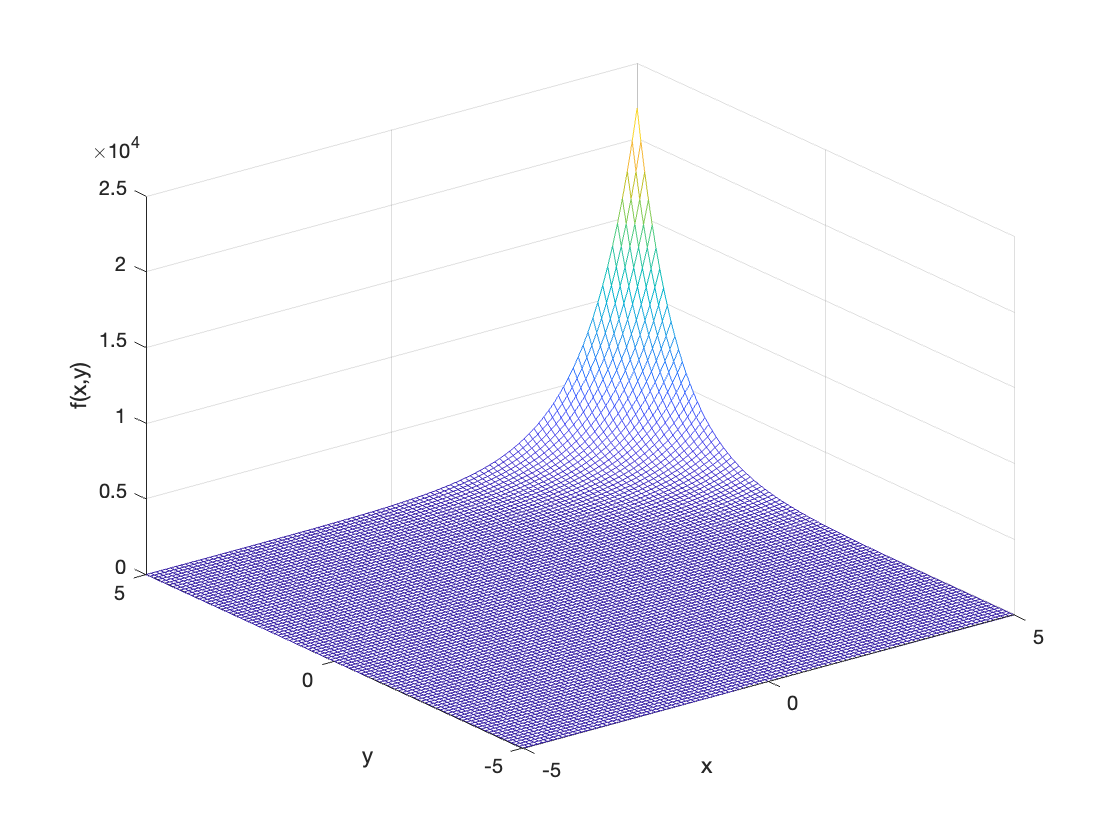
\includegraphics[width=10cm]{przyklad3.png}
\vskip-1.5ex
\caption{Przedstawia wykres funkcji $ f(x,y)=e^{x+y} $.}
\end{figure}
%\nopagebreak
\hfill \break
Funkcja jest bardzo bliska 0 dla $ x+y < 0 $, a w momencie zmiany znaku wykładnika liczby $ e $, gwałtownie wzrasta.
Dla argumentów ujemnych:
 \[
  \lim_{(x,y)\to-\infty} f(x,y)=0, 
  \]
  natomiast dla argumentów dodatnich:
\[
  \lim_{(x,y)\to\infty} f(x,y)=\infty.
  \]
  
\vskip9ex
Wyniki przybliżania przedstawiono w Tablicy 3. 

\begin{table}[h!]
\caption{Wyniki - Przykład 3} \vskip1ex
\renewcommand{\arraystretch}{1.1}
\centering\begin{tabular}{|c|c|c|c|c|}
\hline 	$N$ 		&	$ M $	&	 wynik uzyskany 	& 	wynik teoretyczny	&	błąd  			\\
\hline 	1 		& 	1 		& 	2540.3316 		&	22024.5			&	1.9484e04		\\
\hline 	10 		& 	10 		& 	21139.9826 		& 	22024.5			&	8.8451e02		\\
\hline 	100 		&	100 		& 	22015.2924 		& 	22024.5			&	9.2075			\\
\hline 	1000 	& 	1000 	& 	22024.3740 		& 	22024.5			&	$1.2592e\!-\!01$	\\
\hline 	10000 	& 	10000 	& 	22024.4649 		& 	22024.5			&	$3.5077e\!-\!02$	\\
\hline
\end{tabular}
\end{table}
\vskip2ex

\vskip-2ex
\hfill \break
Podobnie jak w poprzednim przykładzie z każdym kolejnym przybliżeniem błąd jest coraz mniejszy, a uzyskany wynik coraz bliższy wynikowi teoretycznemu.

\subsection{Przykład 4}
Przykład 4 przedstawia przybliżenie bardziej skomplikowanej całki $ \int\limits_{-1}^{1} \int\limits_{-1}^{1}\frac{\sin(10(x^2+y^2))}{10}\,dx\,dy $. \\
Wykres przybliżanej funkcji przedstawia Rysunek 4.
\vskip2ex
\begin{figure}[!h]
\centering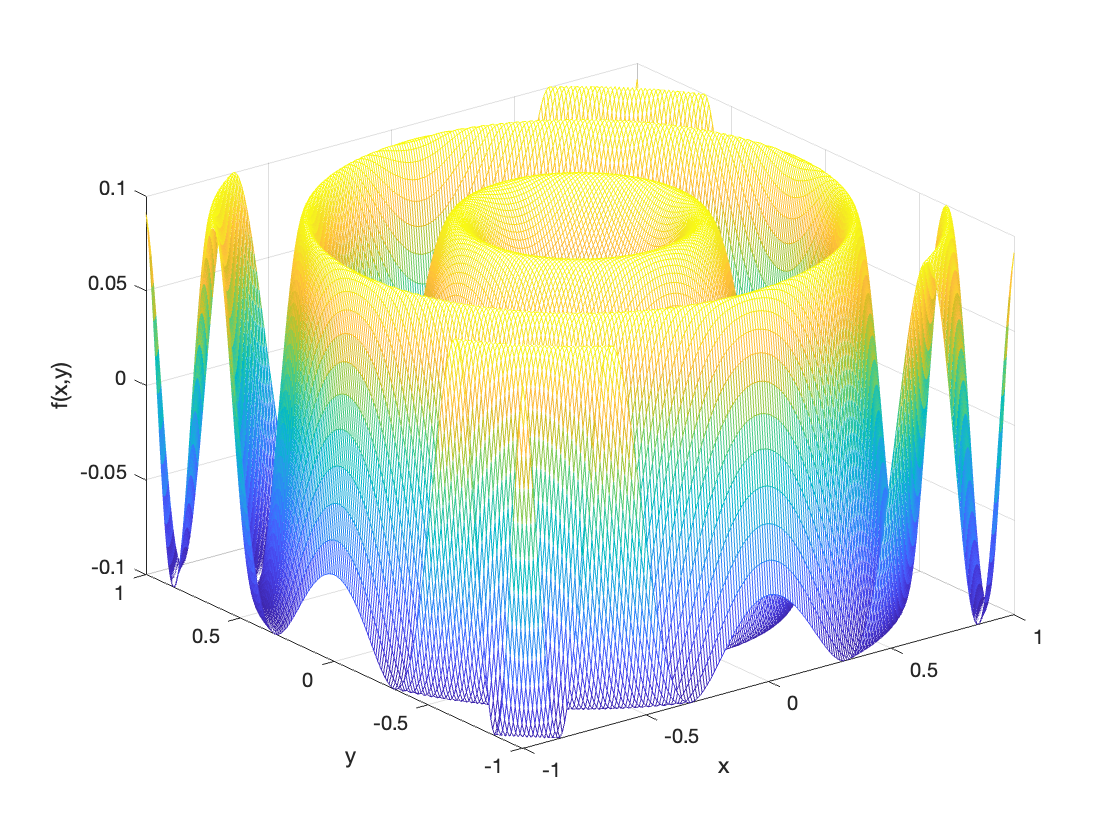
\includegraphics[width=10cm]{przyklad4.png}
\vskip-1.5ex
\caption{Przedstawia wykres funkcji $ f(x,y)=\frac{\sin(10(x^2+y^2))}{10} $.}
\end{figure}
%\nopagebreak
\hfill \break
Funkcja wyglądem przypomina fale kapilarne powstające na powierzchni 2 cieczy. \\
Wyniki przybliżania przedstawiono w Tablicy 4. 

\begin{table}[h!]
\caption{Wyniki - Przykład 4} \vskip1ex
\renewcommand{\arraystretch}{1.1}
\centering\begin{tabular}{|c|c|c|c|c|}
\hline 	$N$ 		&	$ M $	&	 wynik uzyskany 	& 	wynik teoretyczny	&	błąd  			\\
\hline 	1 		& 	1 		& 	-0.0725 			&	0.0334			&	$1.0594e\!-\!01$	\\
\hline 	10 		& 	10 		& 	0.0353 			& 	0.0334			&	$1.9334e\!-\!03$	\\
\hline 	100 		&	100 		& 	0.0334	 		& 	0.0334			&	$1.9760e\!-\!06$	\\
\hline 	1000 	& 	1000 	& 	0.0334	 		& 	0.0334			&	$6.3975e\!-\!08$	\\
\hline 	10000 	& 	10000 	& 	0.0334	 		& 	0.0334			&	$4.5324e\!-\!08$	\\
\hline
\end{tabular}
\end{table}
\vskip2ex

\vskip-2ex
\hfill \break
Mimo, iż wynik teoretyczny jest względnie mały to jako że przedział całkowania jest kwadratem o polu 1, już przy 10 podprzedziałach $ N $ i $ M $ uzyskane wyniki są porównywalne.

\section{Podsumowanie}
Przeprowadzone testy pokazują, że połączenie kwadratury Simpsona i prostokątów daje dokładne lub bardzo niewiele różniące się wyniki niezależnie od zróżnicowania całkowanej funkcji. \\
Metoda jest również efektywna czasowo. Zaimplementowana w Matlabie nie trwa dłużej niż 0.3s nawet przy ilości podprzedziałów rzędu $ 1.0e08 $.

\end{document}  